\documentclass[preprint,12pt]{elsarticle}
\usepackage{graphicx} 
\usepackage{amssymb}
\usepackage{parskip}
\usepackage{tabularx}
\usepackage{xcolor}
\usepackage{caption}
\usepackage{float}
\captionsetup[figure]{font=normalsize}

\usepackage{geometry}

\title{Adsorption of  Sulfonamides  on  phosphorene  quantum dots}
\author{J. W. Pino-Román,  J. D.  Correa,   M.  E.  Mora-Ramos E.  Flórez}
\date{April 2025}

\begin{document}
	
	\maketitle
	
	\section{Introduction}
	
	In recent years, the protection and conservation of water sources have gained enormous significance after decades of negligence in managing the waste produced by human activity. A particular case of this negligence is the biological waste generated by various industries and the rise of antibiotic consumption alongside the increasing human population, which for years has been directly discharged into the water bodies that supply both small and major cities.
	
	Specifically, sulfonamide contamination in water bodies has been a concern, as these water-soluble compounds pose health and environmental risks to both human populations and non-target species \cite{MacLoughlin2024}.
	
	Sulfonamides were discovered in the 1930s as a response to the need for antimicrobials to treat animal bacterial infections, given the increasing demand for animal protein food. After administration, sulfonamides are excreted via urine and feces, subsequently entering the aquatic environment through wastewater discharge, significantly contributing to antibiotic pollution. Despite their relatively low concentrations in environmental samples, measured in $\mu$g/L or ng/L, the continuous release of sulfonamides may pose risks to non-target species previously considered safe, as they can cause unknown effects despite being designed to target specific metabolic pathways, often leading to significant environmental implications \cite{Duan2022}.
	
	The presence of these and various other environmental issues, such as air pollution, has created a need to clean and contribute to the restoration of our vital resources. This is where multiple studies have emerged, aiming to develop structures capable of detecting or adsorbing these pollutants, as their persistence in the environment, particularly in water and soil, poses significant ecological and health risks. Effective decontamination methods are crucial for mitigating these risks. Biochar, particularly when activated with metals like iron, has shown promise in removing sulfonamides from water and soil. Metal-free biochar derived from coconut shells can activate peroxymonosulfate (PMS) to degrade sulfonamides like sulfamethoxazole (SMX) effectively, achieving up to 99\% removal in chloride-rich environments \cite{Hung2021Peroxymonosulfate}. Similarly, iron-activated biochar enhances the sorption of sulfanilamide in soils, reducing its bioavailability and movement, thus mitigating contamination \cite{Gamiz2022The}.
	
	The decontamination of sulfonamides using 2D materials is an emerging area of research, focusing on the development of advanced materials for efficient removal of these antibiotics from water systems. 2D materials, such as covalent triazine-based frameworks and graphitic carbon nitride, have been shown to enhance photocatalytic activity for the degradation of sulfonamides. These materials facilitate charge separation and transfer, leading to high degradation efficiencies under simulated solar light. For instance, a CTFNS/CNNS heterojunction was able to decompose sulfamethazine with a 95.8\% efficiency, highlighting the potential of 2D/2D heterojunctions in wastewater treatment \cite{Cao2020Metal-free}.
	
	Due to their potential, in recent years there has been an increasing interest in the theoretical characterization of 2D materials \cite{Manikandan2019}. For instance, 2D materials are also being utilized in the development of electrochemical immunosensors for the detection of sulfonamides. For example, 2D Cu-TCPP(Fe) has been used to create a highly sensitive sensor capable of detecting sulfonamides at low concentrations. This approach offers a wide detection range and high precision, making it suitable for environmental monitoring \cite{Xiao2019A}.
	
	More recently, quantum dots have gained attention due to their vast number of potential applications. Phosphorene quantum dots \cite{Abdelsalam2019} belong to a new class of zero-dimensional functional nanostructures with unique physicochemical surface properties compared to few-layer phosphorene and other 2D analogues. One of the most interesting applications is the adsorption of various molecules on these phosphorene quantum dots. PQDs are now considered promising catalytic materials for electrocatalytic water splitting and nitrogen reduction, lithium–sulfur batteries, solar light–driven energy devices, and biocatalysis, either in pristine form or as active components for constructing heterostructures with other 2D materials.
	
	\begin{center}
		\begin{figure}[H]
			
			\label{f:Qds}
			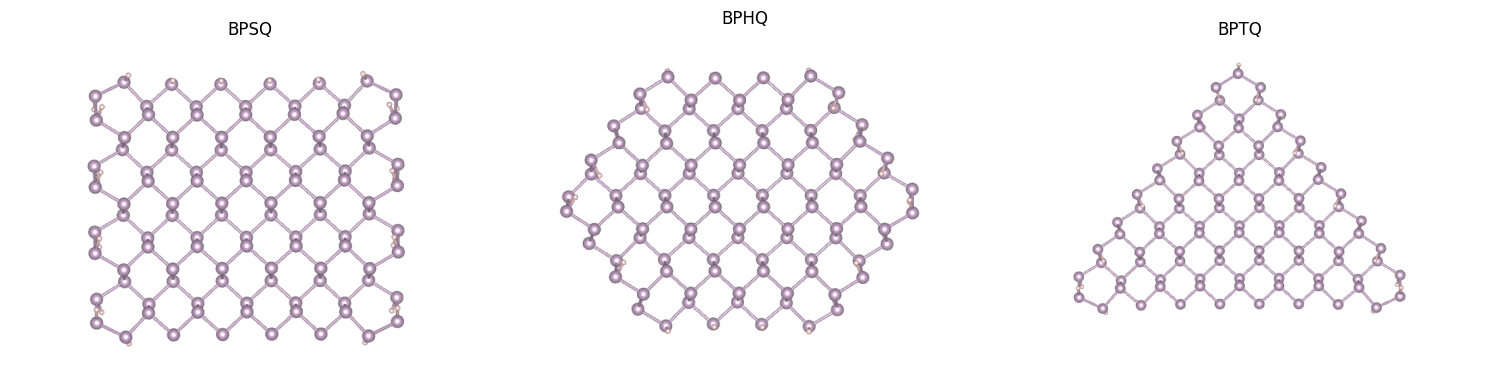
\includegraphics[width=1\textwidth]{quantumDots.png}
			
			\caption{Quantum dot structures for adsorption assessment: Due to the structural differences among the three quantum dots, it is necessary to evaluate potential additional energy contributions from polarizations caused by the edges of each structure.}
			\label{f:Quantum_dots}
		\end{figure}
		
	\end{center}
	
	Motivated by the potential applications of quantum dots in molecule adsorption, we have conducted a systematic study of the electronic properties of phosphorene quantum dots and their adsorption energies for antibiotic contaminants present in water. The calculations were strengthened and corroborated through the use of different exchange-correlation functionals that included van der Waals interactions for adsorption both in the gaseous state and in the presence of a solvent.
	
	\section{Methods and Computational Details}
	
	The methodology employed in this study consists of four main steps: exploration of atomic sites, relaxation of structures, calculation of adsorption energies in gas, and calculation of adsorption energies in solvation.
	
	\subsection{Exploration of Atomic Sites:} Sulfonamides are characterized by two primary structural motifs: five-membered heterocyclic rings and six-membered cyclic structures. The study of sulfate radical-based oxidation processes has emphasized the crucial role of five-membered heterocyclic rings in the degradation of sulfonamides. Additionally, six-membered rings significantly influence the chemical behavior and degradation pathways of these compounds \cite{Zhou2019Sulfate}. Therefore, our exploration focuses on variations in the positioning of these two structures.
	
	To systematically explore adsorption sites, we developed a custom nomenclature for defining six atomic positions on quantum dots (QDs) interacting with sulfonamides. Each site is designated using the format QD-SF-PRS, where:
	
	\textbf{QD} represents the abbreviated name of the quantum dot.\\  
	\textbf{SF} denotes the studied sulfonamide.\\
	\textbf{P} indicates the atomic position.\\
	\textbf{R} specifies the ring type, with values of 5 or 6, corresponding to whether the five- or six-membered ring is parallel to the quantum dot.\\  
	\textbf{S} defines the structural position, with values of 1 for top, 2 for bridge, and 3 for hollow sites.  
	
	For instance, a sulfamethoxazole molecule adsorbed on a triangular phosphorene quantum dot, where the five-membered ring is oriented parallel to the surface and positioned at a top site, is designated as BPTQ-SMX-P51. This classification framework enables a systematic and reproducible exploration of potential adsorption sites on phosphorene quantum dots. This process was conducted using the ASE framework \cite{HjorthLarsen2017}, with the ASE-GUI toolkit for interactive atomic visualization.
	
	\begin{center}
		\begin{figure}[H]
			
			\label{f:DosQD}
			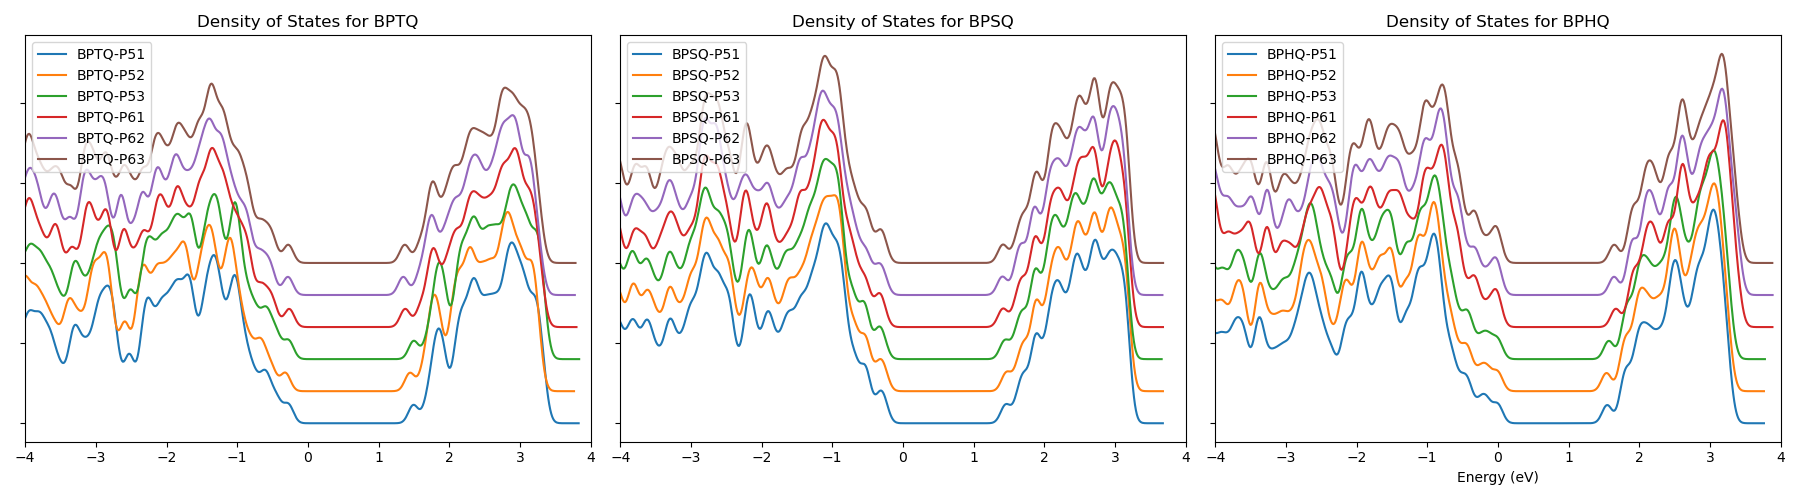
\includegraphics[width=1\textwidth]{density_of_states.png}
			
			\caption{Comparison of the Density of States for the exploring sites: While all three structures exhibit similar general trends, differences in peak positions and intensities suggest variations in electronic properties, potentially influencing conductivity or optical behavior. The overall shape of the DOS curves indicates significant states around ±2–3 eV, with noticeable shifts between the materials, implying structural or compositional effects on their electronic characteristics.}
			\label{f:Dos_QD_ads}
		\end{figure}
		
	\end{center}
	
	
	\subsection{Relaxation of Structures:} Structural relaxation in simulations is essential for accurately predicting adsorption properties, particularly in flexible frameworks such as metal-organic frameworks (MOFs). Rigid models often fail to capture the true adsorption behavior, especially at low concentrations \cite{Yu2021Incorporating}. To ensure the accuracy of our findings, all defined structures were subjected to relaxation using various computational calculators, allowing them to reach their minimum energy configurations. This process is crucial for obtaining reliable adsorption energies and understanding the interactions between quantum dots and antibiotic molecules. This step was performed using the GPAW framework \cite{Mortensen2024} with the linear combination of atomic orbitals (LCAO) calculation mode, considering the ground state for the system of surface and adsorbate, as well as the molecules and quantum dots separately.
	
	\subsection{Calculation of Adsorption Energies in Gas:} First, adsorption energies were calculated for the relaxed structures in the gas phase. This involved determining the energy difference between the isolated quantum dot and antibiotic molecule and the combined system \cite{Correa2024}.
	
	\begin{equation} E_{ads} = E_{complex} - (E_{surface} + E_{adsorbate}) \end{equation}
	
	Where:
	\begin{itemize}
		\item $E_{complex}$ is the total energy of the adsorbate-quantum dot system.
		\item $E_{surface}$ is the energy of the isolated quantum dot. 
		\item $E_{adsorbate}$ is the energy of the isolated adsorbate. 
	\end{itemize}
	
	The calculations were performed using different exchange-correlation functionals to account for van der Waals interactions, which are essential for accurately predicting the properties of materials, especially those involving non-covalent interactions. Traditional DFT methods often fail to capture these interactions, leading to inaccuracies in calculated properties such as adsorption energies and structural parameters \cite{Sevilla2021Graphene-hexagonal}. 
	Among them, we have the Basis set superposition error (BSSE), which arises in quantum chemistry when the energy of a molecular system (especially dimers or complexes) is calculated using basis sets that are not complete. When using a finite basis set, the computed interaction energy can be artificially lowered because the basis set used for a given monomer does not fully account for the basis functions that would be available in the presence of the other monomer. Essentially, each monomer "benefits" from the virtual orbitals of its partner, leading to an apparent reduction in energy which does not represent the true interaction energy when calculated accurately with a complete basis set \cite{Gutowski1993}.
	To analyze the importance of these corrections, the calculations were performed using the PBE exchange and correlation functional, with van der Waals corrections added through the DFDT3 functional \cite{Mahlberg2019Improved}. Given that, the adjusted energy calculation is given by 
	
	\begin{equation} E_{total} = E_{ads} + E_{vdW} \end{equation}
	
	Where the $E_{vdW}$ correction is being calculated with
	
	\begin{equation} E_{vdW} = E_{complex}(DFTD3) - E_{surf}(DFTD3) - E_{adsorbate}(DFTD3) \end{equation}
	
	So this way, to the initial adsorption eneMacLoughlin2024rgy is added the energy correction alculated through van Der Waals functional.
	
	\subsection{Calculation of Adsorption Energies in Solvation:} To simulate more realistic environmental conditions, adsorption energies were also calculated in the presence of a solvent. This step involved using solvation models to account for the interactions between the quantum dots, antibiotic molecules, and the solvent. Efficient implicit solvation models, such as the analytical linearized Poisson-Boltzmann (ALPB) model, are used in semiempirical methods to account for solvation effects. These models provide accurate solvation energies and are computationally efficient, making them suitable for a wide range of systems \cite{Ehlert2021Robust}.
	
	
	\section{Results}
	
	\subsection{Adsorption Dynamics:} During the relaxation calculations, the dynamics of the adsorbate were assessed to determine the most favorable sites for adsorption. However, it was observed that, for each of the quantum dots and configurations, the molecule remained at the original site. The interaction was instead reflected in small deformations in the structure of the surfaces. Accurate start and end points improve the reliability of molecular dynamics simulations and theoretical models, allowing for better predictions of adsorption behavior in various environments, such as liquid-solid interfaces or complex surfaces \cite{Ivanova2024Study} \cite{Cazzaniga2020Anharmonic}.
	
	\begin{figure}[H]
		\centering
		\begin{subfigure}
			\centering
			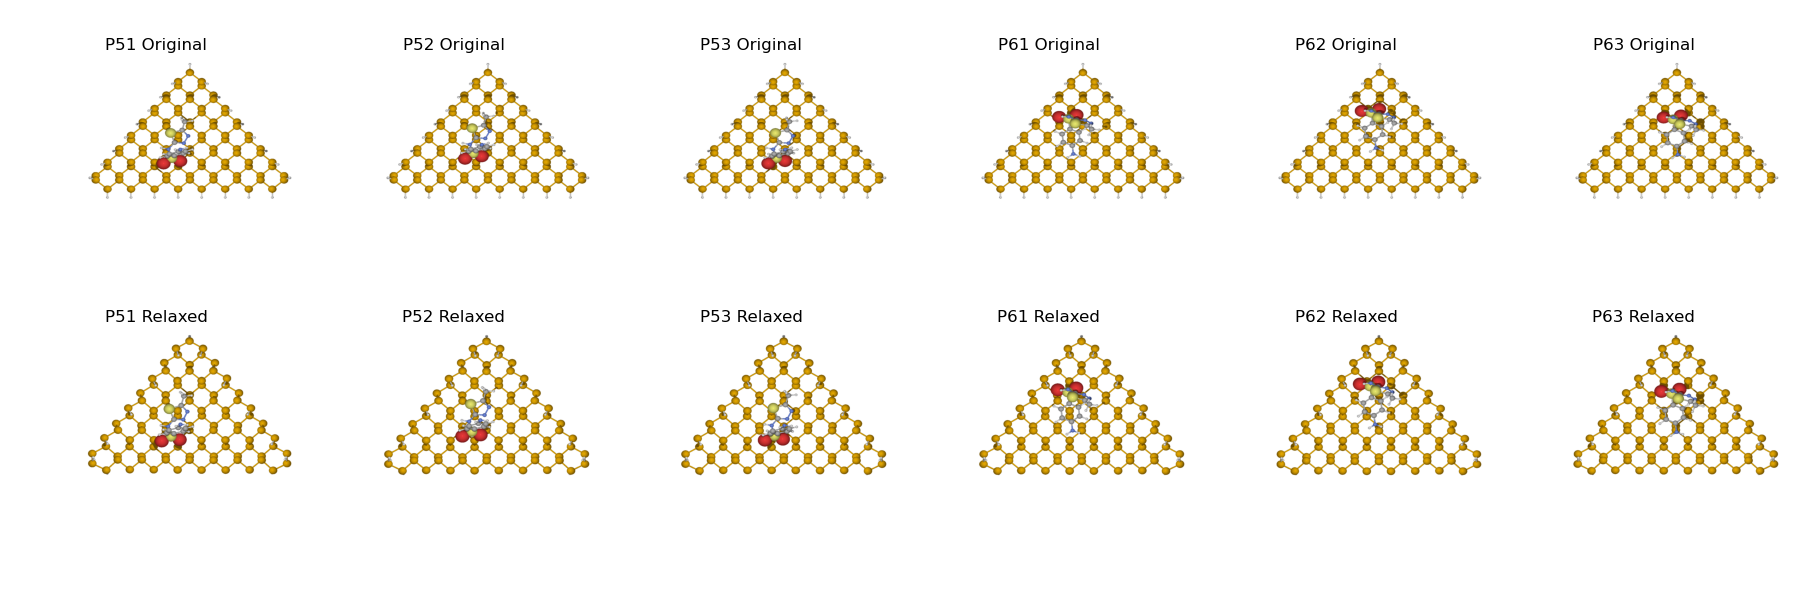
\includegraphics[width=\textwidth]{BPTQArrayplot.png}
			\caption{BPTQ configuration}
			\label{f:BPTQ}
		\end{subfigure}
		
		\begin{subfigure}
			\centering
			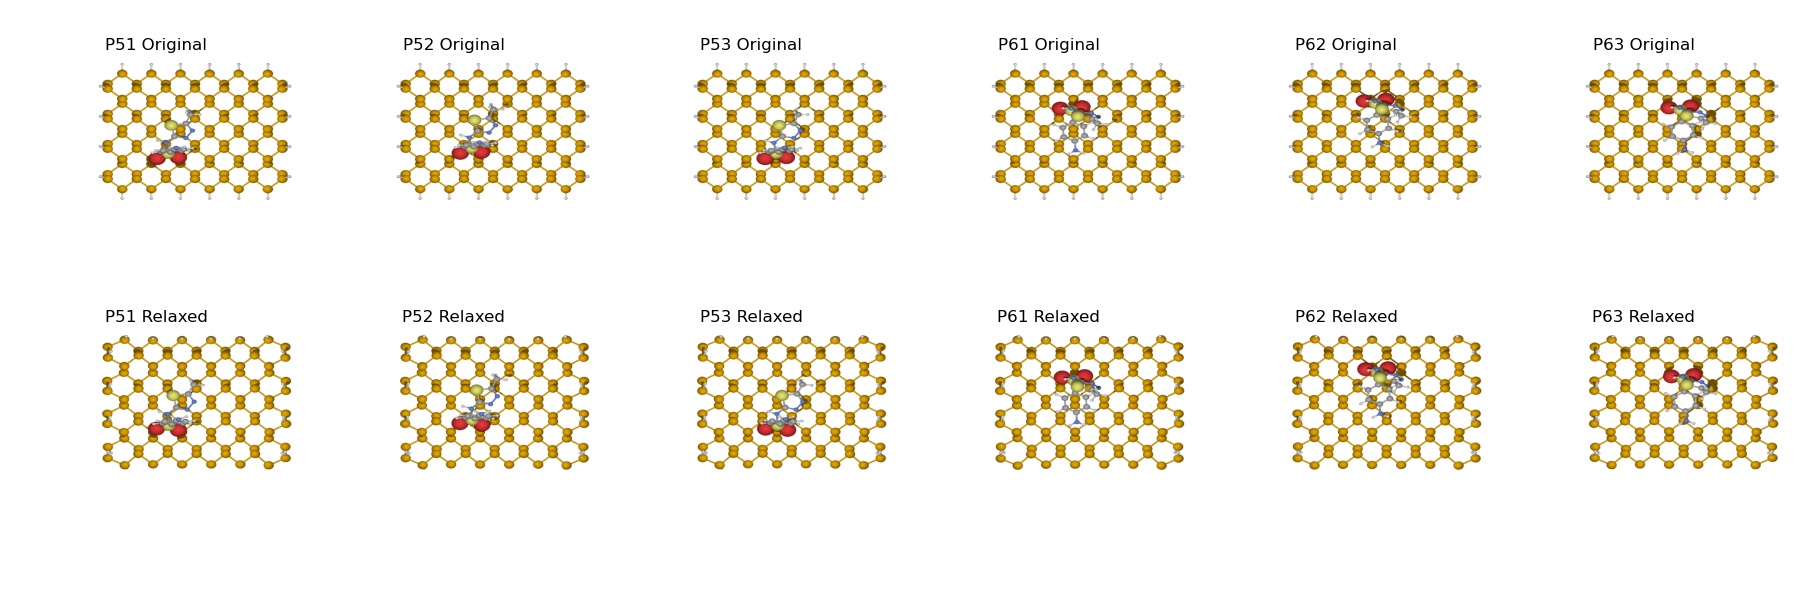
\includegraphics[width=\textwidth]{BPSQArrayplot.png}
			\caption{BPSQ configuration}
			\label{f:BPSQ}
		\end{subfigure}
		
		\begin{subfigure}
			\centering
			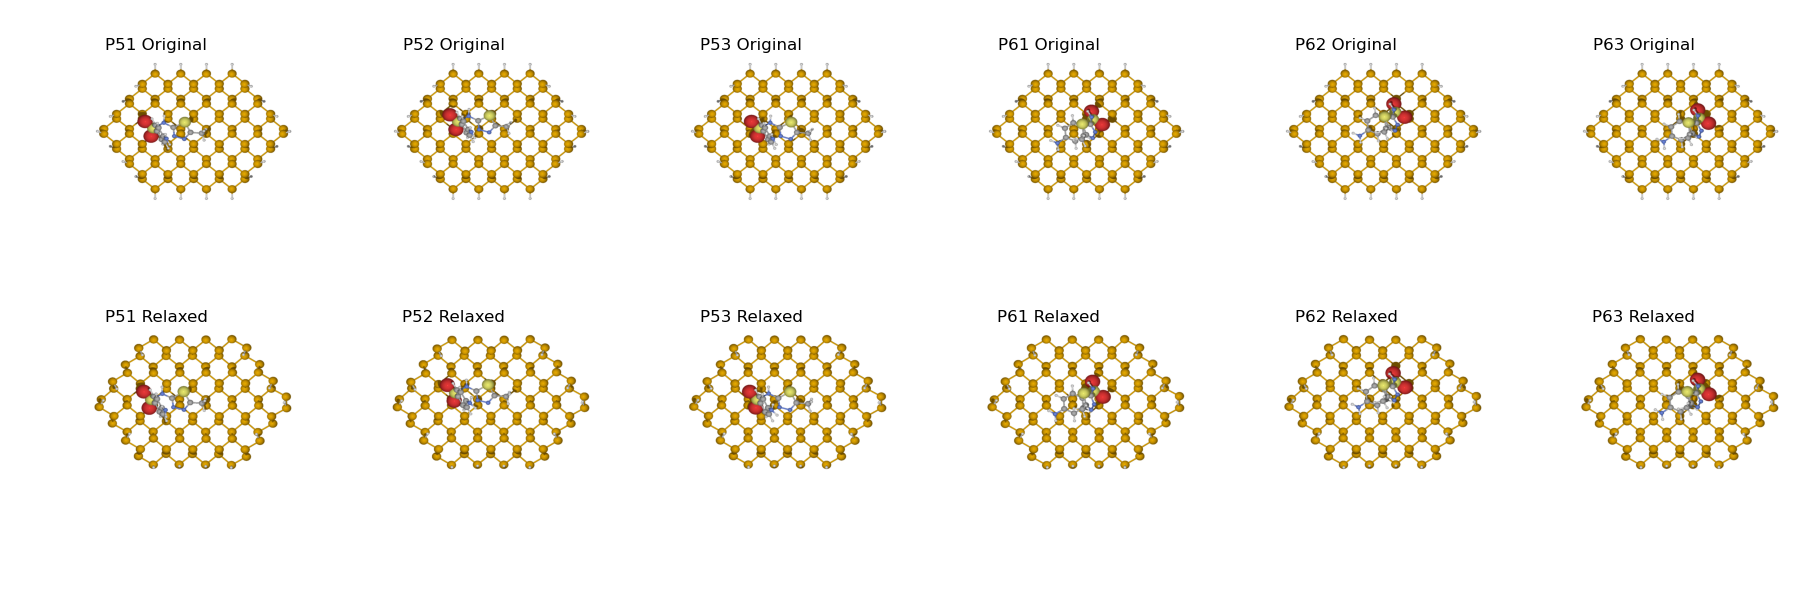
\includegraphics[width=\textwidth]{BPHQArrayplot.png}
			\caption{BPHQ configuration}
			\label{f:BPHQ}
		\end{subfigure} 
		\caption{Begin and end point for every configuration over every quantum dot}
		\label{f:Dos_Multiple}
	\end{figure}
	
	\subsubsection{Structural Stability Assessment}
	The comparative visualization in Figure~\ref{fig:relaxation} reveals three key findings regarding the relaxation process:
	
	\begin{itemize}
		\item \textbf{Lattice Invariance}: The substrate lattice parameters remain unchanged, with negligible variation in interatomic distances.
		
		\item \textbf{Adsorbate Stationarity}: Adsorbed sulfamethazine molecules exhibit minimal displacement.
		
		\item \textbf{Site Preservation}: All molecular configurations maintain their original adsorption sites (top/bridge/hollow) with minimal positional deviations.
	\end{itemize}
	
	\subsubsection{Implications of Structural Rigidity}
	The observed stability suggests:
	
	\begin{enumerate}
		\item \textbf{Near-Equilibrium Initial Conditions}: The pre-relaxation structures were already within the local energy minimum \cite{Alamatian2013Displacement-based}.
		
		\item \textbf{Symmetry-Governed Stability}: The symmetry of both phosphorene quantum dots and sulfamethazine molecules appears to minimize configurational degeneracy \cite{Yang2014Reversible}.
	\end{enumerate}
	
	
	
	\subsection{Density of states}
	
	\begin{center}
		\begin{figure}[H]		
			\label{f:DosMax}
			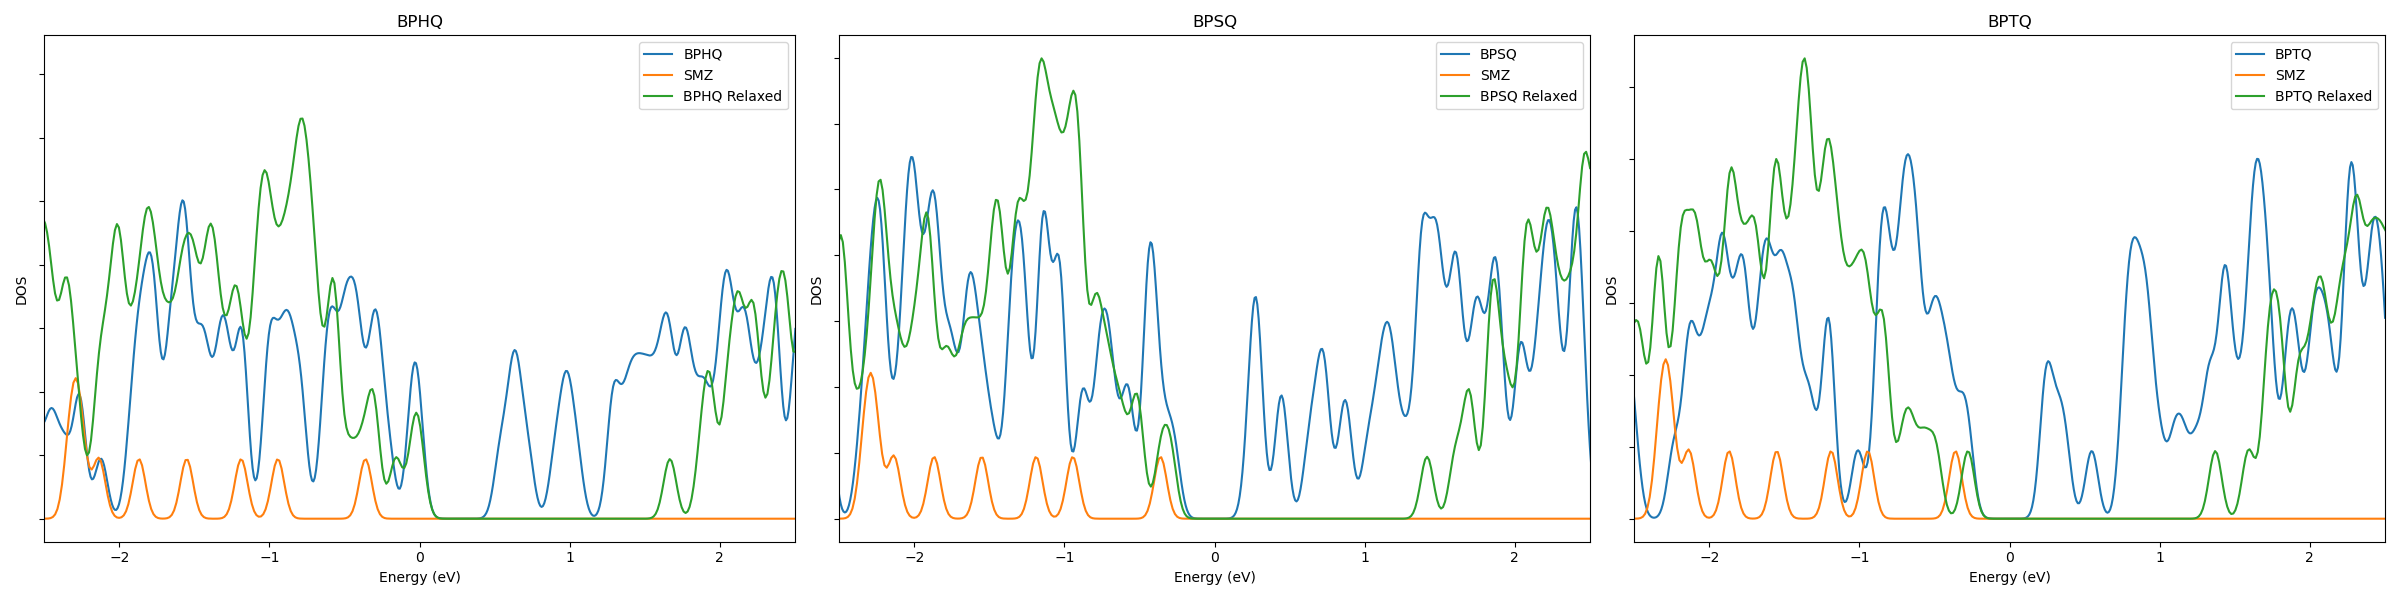
\includegraphics[width=1\textwidth]{Multiple-DoS-QD.png}
			
			\caption{Density of States for the configurations with the strongest adsorption energy. Green curve represents the DoS of the relaxed total system with the adsorbate and the molecule. Orange and blue represent the isolateds molecule and surface respectively.}
			\label{f:Dos_Max_ads}
		\end{figure}
		
	\end{center}
	
	The green DOS includes both the main molecule and SMZ, meaning the electronic states arise from both species interacting. The trend is consistent for BPHQ, BPSQ, and BPTQ, meaning the hybridization effect between each of these molecules and SMZ follows a similar pattern.
	
	The most noticeable differences appear near the Fermi level (E ≈ 0 eV), which suggests that SMZ could alter the transport or conductivity properties of the system.
	
	In certain energy regions, the green curve has features that do not appear in the blue curve, meaning new electronic states emerge in the presence of SMZ.
	
	
	\subsection{Adsorption energies}
	
	\begin{table}[H]
		
		\begin{center}
			\caption{Adsorption energy values for SMZ on PQDs}
			\label{tab:all_configs}
			
			\begin{tabular}{| c | c | c | c | c |}
				\hline
				- & \multicolumn{2}{|c|}{vdW-DF2} & \multicolumn{2}{|c|}{DFTD3}  \\
				
				\hline
				Configuration & Eads Gas (eV) & Eads Water (eV) & Eads Gas (eV) & Eads Water (eV) \\
				\hline
				BPSQ-SMZ-P51&  -0.691 & -0.566 & -0,781 & -0,647\\
				BPSQ-SMZ-P52&  -0.696 & -0,547 & -0,757 & -0,606\\
				BPSQ-SMZ-P53&  -0.681 & -0,543 & -0,770 & -0,638\\
				BPSQ-SMZ-P61&  -0.668 & -0,646 & -0,862 & -0,782\\
				BPSQ-SMZ-P62&  -0.715 & -0,606 & -0,830 & -0,700\\
				BPSQ-SMZ-P63&  -0.618 & -0,583 & -0,759 & -0,707\\
				BPHQ-SMZ-P51&  -0.668 & -0,531 & -0,828 & -0,670\\
				BPHQ-SMZ-P52&  -0.659 & -0,517 & -0,676 & -0,587\\
				BPHQ-SMZ-P53&  -0.649 & -0,511 & -0,669 & -0,561\\
				BPHQ-SMZ-P61&  -0.746 & -0,629 & -0,799 & -0,686\\
				BPHQ-SMZ-P62&  -0.654 & -0,602 & -0,687 & -0,656\\
				BPHQ-SMZ-P63&  -0.671 & -0,578 & -0,762 & -0,695\\
				BPTQ-SMZ-P51&  -0.635 & -0,489 & -0,753 & -0,608\\
				BPTQ-SMZ-P52&  -0.621 & -0,452 & -0,719 & -0,561\\
				BPTQ-SMZ-P53&  -0.638 & -0,456 & -0,767 & -0,604\\
				BPTQ-SMZ-P61&  -0.709 & -0,557 & -0,910 & -0,751\\
				BPTQ-SMZ-P62&  -0.733 & -0,567 & -0,844 & -0,689\\
				BPTQ-SMZ-P63&  -0.661 & -0,534 & -0,847 & -0,706\\
				\hline
			\end{tabular}
			
		\end{center}
	\end{table}
	
	
	The calculated adsorption energy values, ranging from $-0.452$ to $-0.910$ eV, confirm that phosphorene quantum dots (PQDs) exhibit strong interactions with sulfamethazine (SMZ). The negative values indicate energetically favorable adsorption across all configurations \cite{Khnifira2021Combined}. Table \ref{tab:top_configs} summarizes the most and least stable configurations:
	
	\begin{table}[h]
		\centering
		\caption{Extreme adsorption energy values for SMZ on PQDs}
		\label{tab:top_configs}
		\begin{tabular}{lcccr}
			\toprule
			\textbf{Property} & \textbf{Configuration} & \textbf{Functional} & \textbf{Phase} & \textbf{$E_{ads}$ (eV)} \\
			\midrule
			Strongest adsorption & BPTQ-SMZ-P61 & DFTD3 & Gas & $-0.910$ \\
			Strongest in water & BPSQ-SMZ-P61 & DFTD3 & Water & $-0.782$ \\
			Weakest adsorption & BPTQ-SMZ-P52 & vdW-DF2 & Gas & $-0.621$ \\
			Weakest in water & BPTQ-SMZ-P52 & vdW-DF2 & Water & $-0.452$ \\
			\bottomrule
		\end{tabular}
	\end{table}
	
	\subsection{Key Trends and Observations}
	
	\subsubsection{Effect of van der Waals Corrections}
	The choice of dispersion correction significantly impacts the results:
	\begin{itemize}
		\item DFTD3 predicts consistently stronger adsorption than vdW-DF2 (e.g., BPTQ-SMZ-P61: $-0.709$ eV vs $-0.910$ eV in gas phase)
		\item Energy differences of 10--25\% highlight the importance of proper dispersion treatment
	\end{itemize}
	
	\subsubsection{Solvent Effects}
	The aqueous environment reduces adsorption strength:
	\begin{itemize}
		\item Energies are 5--30\% weaker in water (e.g., BPTQ-SMZ-P51: $-0.753$ eV $\rightarrow$ $-0.608$ eV)
		\item Exception: BPSQ-SMZ-P61 shows minimal reduction ($-0.668$ eV $\rightarrow$ $-0.646$ eV), suggesting particular stability
	\end{itemize}
	
	\subsubsection{Structural Dependencies}
	\begin{figure}[h]
		\centering
		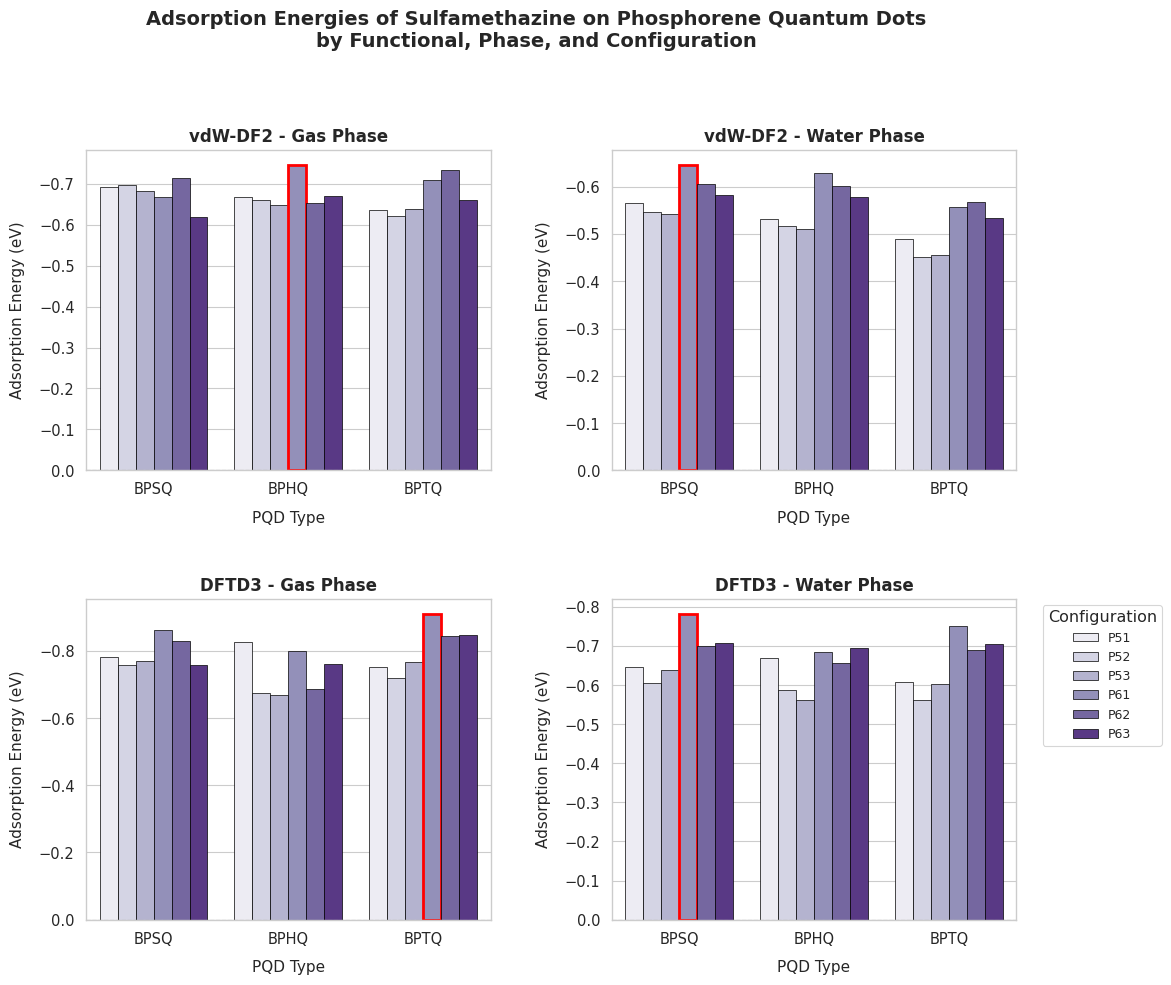
\includegraphics[width=0.8\linewidth]{resumeTable.png}
		\caption{Comparison of adsorption energies by PQD geometry and binding site}
		\label{fig:pqd_comparison}
	\end{figure}
	
	The data reveal clear structural trends:
	\begin{itemize}
		\item \textbf{PQD Geometry}:
		\begin{itemize}
			\item Triangular (BPTQ) shows strongest adsorption (e.g., $-0.910$ eV for P61)
			\item Hexagonal (BPHQ) intermediate ($-0.799$ eV)
			\item Square (BPSQ) most consistent across configurations
		\end{itemize}
		
		\item \textbf{Binding Site Preference}:
		\begin{itemize}
			\item Six-membered ring (P6X) generally outperforms five-membered (P5X)
			\item Hollow sites (P53/P63) more stable than top/bridge sites in water
		\end{itemize}
	\end{itemize}
	
	\subsection{Implications for Applications}
	The results suggest several important considerations for practical implementation:
	\begin{itemize}
		\item Triangular PQDs (BPTQ) with six-membered ring adsorption (P61/P63) are optimal candidates
		\item The robustness of BPSQ configurations in aqueous environments makes them attractive for water treatment
		\item DFTD3 should be used for accurate adsorption energy predictions
	\end{itemize}
	
	
	\section{Conclusions}
	
	Efficacy of Phosphorene Quantum Dots (PQDs) for Sulfonamide Adsorption. 
	The study demonstrates that phosphorene quantum dots (PQDs) exhibit significant potential for adsorbing sulfonamide antibiotics from aqueous environments. The calculated adsorption energies, particularly when accounting for van der Waals interactions, suggest strong interactions between PQDs and sulfonamide molecules. This highlights PQDs as promising candidates for water decontamination technologies, especially in scenarios where low-concentration pollutants persist.
	
	DFTD3-calculated adsorption energies reveal that triangular PQDs (BPTQ) with six-membered ring orientations (e.g., P61) exhibit the strongest affinity for sulfamethazine (−0.910 eV in gas phase), making them optimal for antibiotic capture.
	
	Solvation reduces adsorption energies by up to 30\%, but configurations like BPSQ-SMZ-P61 maintain robustness (−0.782 eV in water), highlighting their potential for real-world water remediation.
	
	The dominance of hollow sites and six-membered ring interactions underscores the importance of atomic-scale tailoring in PQD design for pollutant removal.
	
	
	
	Impact of Solvation and Environmental Conditions
	The inclusion of solvation models in the calculations provided insights into the adsorption behavior under realistic environmental conditions. While the gas-phase results were informative, the solvation studies are crucial for translating these findings into practical applications, as they account for the complex interactions in aqueous systems. Future work could explore the effects of varying pH, temperature, and ionic strength on adsorption efficiency.
	
	Compared to other 2D materials and biochar-based solutions, PQDs offer unique advantages, such as tunable electronic properties and high surface-to-volume ratios. The study’s results align with emerging research on 2D materials but emphasize the distinct potential of PQDs due to their zero-dimensional nanostructure and versatility in forming heterostructures.
	
	To bridge the gap between theoretical predictions and practical applications, experimental validation of these computational findings is essential. Additionally, investigating the recyclability and stability of PQDs in real-world water treatment systems could further validate their suitability for large-scale environmental remediation.
	
	\newpage
	
	\bibliographystyle{unsrt}
	\bibliography{references.bib}
\end{document}

